
\section{Accelerators and Detectors: the LHC and the CMS}
\label{sec:org3878a16}
\subsection{The Large Hadron Collider}
\label{sec:org5906b28}
Our knowledge in the field of high energy physics has been largely obtained through fixed target experiments that used proton and electron accelerators. However, over the last decades, the significance of colliding beam experiments has been rising. Such experiments involve two particle beams that rotate in opposite directions and collide at multiple points around the ring. The key advantage of colliding beam machines is their ability to produce new particles due to the high center of mass energy created during the collision. This energy increases linearly as E, rather than as \(E^{1/2}\), in fixed target experiments, and almost all of it is utilized in generating new particles\cite{thomson_2013}.

One great example of a colliding beam machine is The Large Hadron Collider (LHC).  The LHC has been instrumental in many groundbreaking discoveries, with the most famous one beeing the Higgs boson, and has helped scientists to further our understanding of the fundamental nature of the universe. The LHC encompasses a 27-kilometre ring consisting of superconducting magnets with numerous accelerating structures along its length.

Within the accelerator, a strong magnetic field is accelerating the two counterrotating proton beams to velocities near that of the speed of light uppon collision.  The thousands of  superconducting magnets, responsible of the generation of the magnetic field, are of varying sizes and types. Dipole magnets, 1232 in total and 15 meters in length, are utilized to bend the beams and quadrupole magnets, 392 in total and 5-7 meters long, focus the beams. Prior to collision, another type of magnet is used to compress the particles, increasing the likelihood of collisions \cite{MomentumCMS}
\subsection{The Compact Muon Solenoid}
\label{sec:orgccfbfe1}
The main goal of  the Compact Muon Solenoid (CMS), as a general purpose particle detector, is to  to reconstruct the Feynman diagram associated with any interaction that might happen inside the LHC. The first and foremost interactions that happen are the collisions between the beams, which generate individual interactions known as \emph{events}. Even though most of the particles associated with an event are unstable, their final decay products, are stable enough to reach the detector and be measured. In the rest of the chapter I will give a brief overview of the CMS detector and discus how does it detect particles.
\subsubsection{Overview}
\label{sec:org3cfeb42}
The CMS detector consists of 5 compartments, each with unique functionality, that are organised in several coaxial layers. The Silicon Tracker, located in the innermost part of CMS, includes silicon pixel vertex detectors and silicon strip detectors, which trace the position and momentum of charged particles. The Electromagnetic Calorimeter (ECAL), the second layer, is composed of PbWO4 crystals and intended to detect photons and electrons. The Hadronic Calorimeter (HCAL), the third layer, is designed to identify hadrons. The Superconducting Solenoid Magnet, the fourth layer, is an solenoid coil that generates a constant magnetic field of 4 T along the direction of the  beam. Due to the deflection of the trajectories of charged particles by the magnet, it becomes possible to measure their momentum. The final, outer most layer, is responsible for the measurement of muon the tracks. Figure \ref{fig:CMS_detector}\cite{CMSDetectorOverview} provides a sectional view of the CMS detector.
\begin{figure}[hb]
\centering
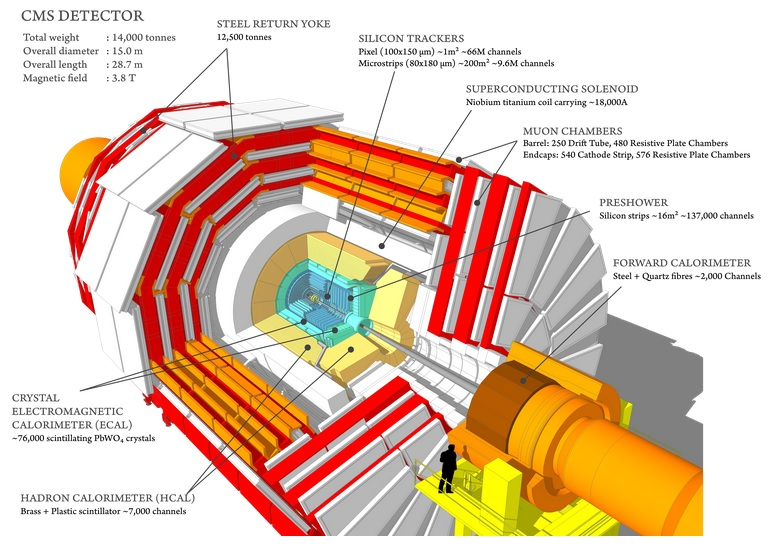
\includegraphics[width=0.8 \textwidth, ext=.png type=jpg]{/home/kpapad/UG_thesis/Thesis/Dissertation/src/figures/cms_detector.jpg}
\caption{A cross-sectional perspective of the CMS detector}
\label{fig:CMS_detector}
\end{figure}

\subsubsection{Coordinate convention at the CMS}
\label{sec:orge8fa37a}
Given the solenoid geometry of the CMS detector, it is more convenient to use a spherical type of coordinates\(\left(r, \phi, \theta \right)\). The origin is located at the collision point and the z axis is parallel to the beam as shown in figure \ref{fig:CMSCoords}. In this system, the momentum of a particle(or any other vector) can be analyzed in a component parallel to the z axis and one component perpendicular to the z axis(Transverse mometnum). Transverse mometnum is defined as follows:
\begin{equation}
|\vec{P_{T}}| = \sqrt{P_{x}^{2} + P_{y}^{2}} = |\vec{P}|\sin{\phi}
\end{equation}
Where \(|\vec{P}| = \sqrt{P_{x}^{2} + P_{y}^{2} + P_{z}^{2}}\). The CMS detector, measures the transverse energy\cite{MomentumCMS} of particles, and thus it is useful to work with the transverse momentum \(P_{T}\). The azimuth angle  \(\phi \in \left[0, 2\pi\right)\) coordinate is the angle between \(P_{t}\) and x axis and the polar angle  \(\theta \in \left[0, \pi   \right]\) is the angle between the momentum vector and the z axis.

\begin{figure}[ht]
\centering
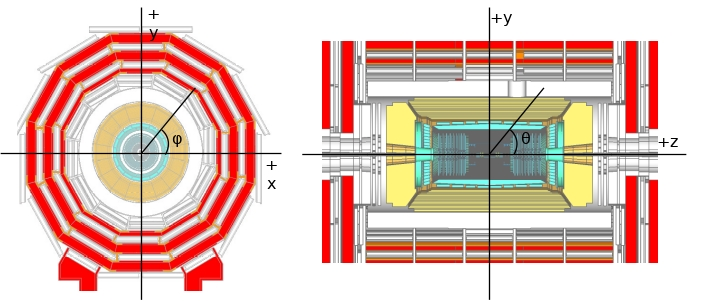
\includegraphics[width=0.7 \textwidth, ext=.png type=jpg]{/home/kpapad/UG_thesis/Thesis/Dissertation/src/figures/cms_coords.jpg}
\caption{CMS coordinates}
\label{fig:CMSCoords}
\end{figure}


Due to the relativistic nature of the phenomena taking place inside LHC, it is more usefull to work with lorentz invariant quantities \cite{AcceleratorsLecture}. Thus, instead of working with the polar angle it is more convenient to introduce the lorentz invariant  \emph{pseudorapidity} \(\eta\in \left [ -\infty, +\infty \right ]\).  Pseudorapidity is defined as:
\begin{equation}
\eta \equiv -\ln{\left [ \tan\left (\frac{\theta}{2} \right ) \right]  }
\end{equation}

The cartesian\(p_{x}\text{, } p_{y}\text{, }p_{z}\) momentum components are related to the \(P_{T}\text{, }\eta\text{, }\phi\)  components by the following transformation relations:
\begin{equation}
\begin{matrix}
p_{x} = P_{T}\cos{\phi} \\
p_{y} = P_{T}\sin{\phi} \\
p_{z} = P_{T}\sinh{\eta}\\
|\vec{P}| = P_{T}\cosh{\eta} 
\end{matrix}
\end{equation}

\subsubsection{Position tracking and momentum measurements: Silicon Tracker}
\label{sec:org2c477d8}
The Silicon tracker measures the positions of charged particles at a number of points, thus it is able to record their trajectory. Given the radius of curvature of the particle's track(due to the 4T magnetic field of the super conducting solenoid), the tracker provides sufficient information, to reconstruct the momentum of the particle. More over, the geometrical location of the trajectory gives direct information regarding the position of the particle. Therefore, the silicon tracker measurements  provide  information regarding the \(P_{T}\text{, } \eta\text{ and }\phi\) of the particles that it detects.

\begin{figure}[ht]
\centering
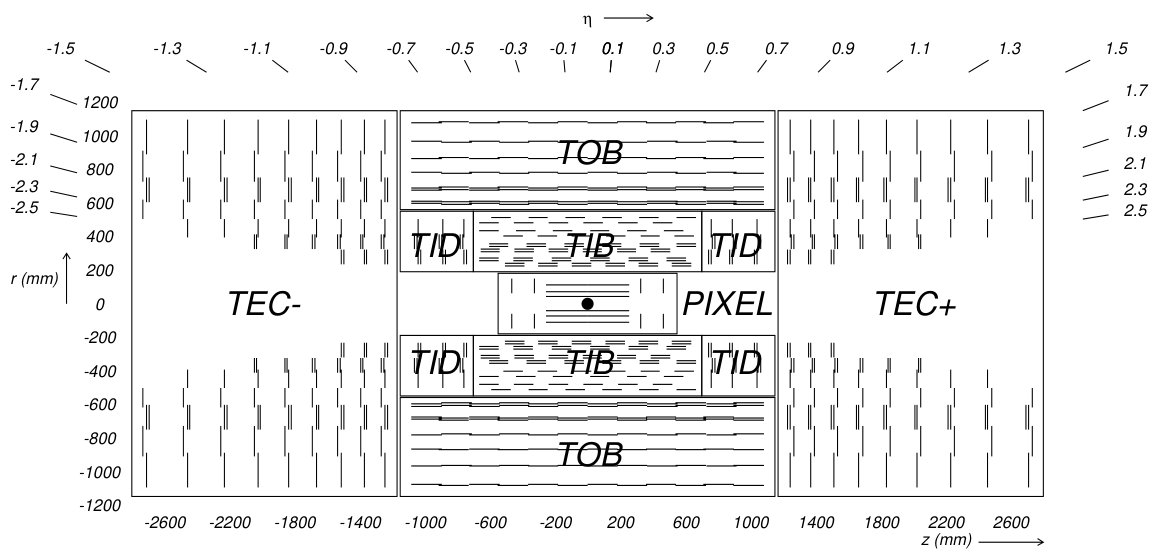
\includegraphics[width=0.9 \textwidth, ext=.png type=jpg]{/home/kpapad/UG_thesis/Thesis/Dissertation/src/figures/cms_tracker.jpg }
\caption{Schemtic illustration of a crossection of the CMS Tracker }
\label{fig:si_tracker}
\end{figure}


A schematic representation of the Sillicon Tracker's corss section, can be viewed on figure \ref{fig:si_tracker}\cite{Chatrchyan:1129810}. The tracker consists of a silicon pixel detector and a silicon strip detector. The silicon pixel detector is composed of two sub-detectors. Namely, the barrel which consists of three layers covering the region \(|\eta| < 2.2\) and at \(r = 4.4\text{, }7.3\text{ and }10,2\text{cm}\). The end caps, are two discs of pixel modues, located one on each side, that complete the design of the silicon pixel detector. The pixel detector improrves the trajectory and position measurements, by providing two-dimensional measurements of the charged particles' hit positions.

The silicon strip detector, covers the radial region \(r \in \left[ 20, 116 \right]\text{cm}\). and  is comprised of four inner barrel (TIB) layers and two inner endcaps (TID). The TIBs are assembled in shells and each TID consists of three small discs. The outer barrel (TOB) encompasses both TIB and TID and contains six concentric layers. The tracker is closed off on either end by two endcaps (TEC). Measurements at the silicon strip detector give information regarding the path of each particle allows the distinction of separate particle trajectories.

\subsubsection{Energy Measurements: Calorimeters}
\label{sec:orgeca8eed}
Apart from measuring position and momentum, determining the energy of particles produced in LHC collisions is crucial. In the Compact Muon Solenoid (CMS) experiment, this information is obtained from particle interactions with matter in the calorimeters. Particles that are stable enough to reach the detector without decaying are either leptons, photons, or hadrons. The interactions between electrons, photons, and matter are of electromagnetic nature, while those between hadrons (charged or neutral) and matter are strong interactions. Therefore, the CMS experiment employs two types of calorimeters: the Electromagnetic Calorimeter (ECAL), located at the innermost layer, which measures the energy of photons and electrons, and the Hadron Calorimeter (HCAL), situated at the outer shells of the calorimeter section.

\begin{itemize}
\item Electromagnetic Calorimeter (ECAL)
\label{sec:org54126fa}

Figure \ref{fig:cms_ecal}\cite{mac-2014}, provides a view of the Electromagnetic calorimeters inside the CMS. The ECAL is composed of lead tungstate (PbWO4) crystals and is designed with a central barrel section (EB) and two endcaps (EE) that cover a range of pseudorapidities up to \(1.48\leq|\eta| \leq 3.0\)\cite{Biino_2015}. The crystals are highly dense and scintillate when high-energy photons or electrons interact with them. When a particle passes through the ECAL, it deposits its energy in the form of electromagnetic showers, which cause the crystals to emit light. The emitted light is then captured and amplified in order to estimate the energy of the incoming particle. The high-density crystals of the ECAL make it possible to accurately measure the energy of photons and electrons with high precision and resolution. 

\begin{figure}[ht]
\centering
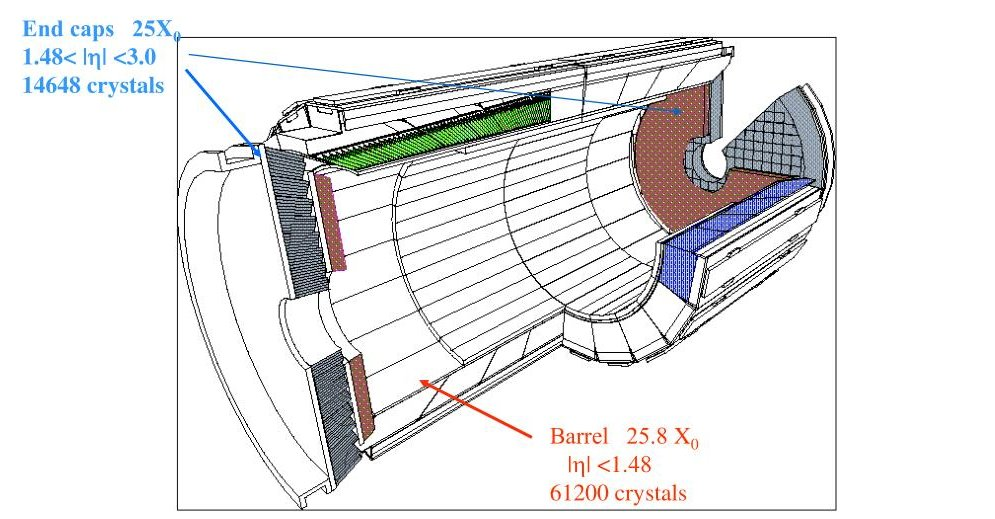
\includegraphics[width=0.9 \textwidth, ext=.png type=jpg]{/home/kpapad/UG_thesis/Thesis/Dissertation/src/figures/cms_ecal.jpg }
\caption{Schemtic illustration of the Ecal parts inside CMS }
\label{fig:cms_ecal}
\end{figure}


\item Hadron Clorimeter (HCAL)
\label{sec:orgbfeffb5}

The hadrons that manage to reach the detector, fly off the ECAl and interact with the Hadron Calorimeter. The HCAL consists of alternating layers of absorber material and plastic scintillator tiles that detect particles generated by the hadrons as they interact with the absorber.  When particles pass through the HCAL, they interact with the absorber material, producing showers of particles that create signals in the scintillator tiles. These signals are then read out and processed to measure the energy of the incoming hadrons. The HCAL has both a barrel section(HB), with pseudorapidity coverage at \(|\eta|<1.3\) and endcap(HE), covering a range of pseudorapidities \(1.3\leq|\eta| \leq 3.0\). The HCAL is highly effective at measuring the energy of hadrons due to its high-density absorber material and precise arrangement of scintillator tiles\cite{HcalLecture}
\end{itemize}

\subsubsection{Detecting Muons}
\label{sec:org8c95f86}
In the outer regions of the CMS detectors, are located the muon chambers. They are the final part of the detector and are designed soley for the detection of muons, which due to their large mass(207 times greater than the electron mass) muons travel a longer distance in matter than electrons. Thus, their energy cannot be measured in ECAL. 

The muon chambers consist of 250 drift tubes (DTs) and 540 cathode strip chambers (CSCs), which track the positions of the particles. Additionally, there are 610 resistive plate chambers (RPCs) and 72 gas electron multiplier chambers (GEMs), making a total of 1400 chamber units . The use of multiple layers of detectors and different types of chambers makes the system robust and able to filter out background noise.

\begin{figure}[ht]
\centering
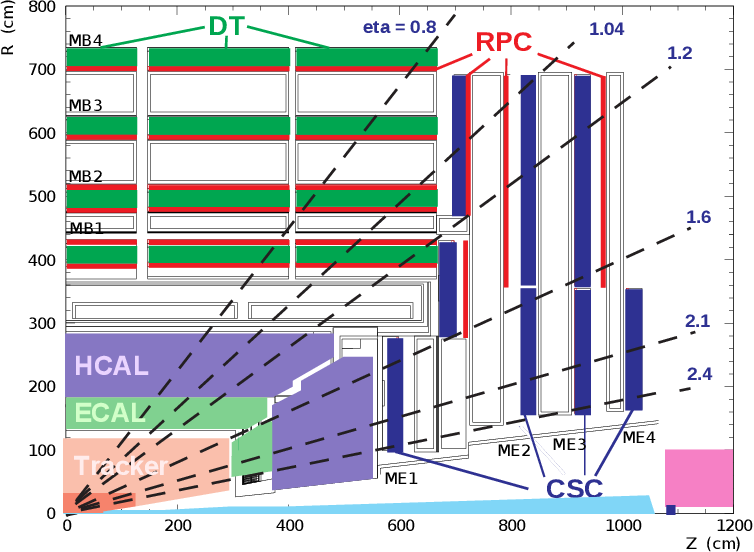
\includegraphics[width=0.9 \textwidth, ext=.png type=png]{/home/kpapad/UG_thesis/Thesis/Dissertation/src/figures/cms_MuonChambers.png }
\caption{A quarter sectional view of the CMS muon chambers. The beamline is perpendicular to the plane of the page}
\label{fig:muon_chambers}
\end{figure}

Figure \ref{fig:muon_chambers} illustrates the arrangement of the four different kinds of chambers. In the "barrel region," which surrounds the beam line, the DTs and square-shaped RPCs are grouped in coaxial cylinders. The CSCs, trapezoidal RPCs, and GEMs are located at the end cap region of the barrel . This arrangement allows for accurate measurements of the muons' trajectories and momenta in different regions of the detector.\cite{CMSDetectingMuons}
\subsection{Event Reconstruction \& Detector Calibration}
\label{sec:org3fecb86}
\subsubsection{Event Reconstruction}
\label{sec:orgfae79d0}
The infrastructure described in the previous sections provides (almost) all the necessary information regarding the particle collisions taking place inside the LHC. The next step is to combine this information to reconstruct the physical objects (particles, jets, etc.) that are being produced in each collision (event).

As already discussed, the trajectories and momenta of the charged particles are reconstructed using information coming from the pixel tracker, while signals coming from the calorimeters provide energy measurements of the particles. The Particle Flow algorithm is then used to combine information from all subdetectors to create a consistent set of physical objects, including electrons, photons, muons, and neutral and charged hadrons. These objects are further processed by dedicated algorithms to reconstruct composite objects such as taus and jets, and to estimate missing energy. To determine the vertices of the collisions, information from the reconstructed tracks of the particles is used. The primary vertex is defined as the vertex with the largest sum of the transverse momentum of all contributing physical objects.
\subsubsection{Callibration and energy scale uncertainties}
\label{sec:org41e8e4d}
The reconstructed objects, are usually calibrated using well-known resonances, such as the Z boson or J/psi meson, whose masses and decay properties are well-measured. The calibration process involves adjusting the energy scale and resolution of the reconstructed objects such that the resonances in data and simulation appear at the correct mass values with the correct amount of smearing.

However, it is not possible to achieve a perfect agreement between data and simulation due to the complexities of the subdetectors and reconstruction algorithms used in the experiment, as well as nonlinear effects such as detector aging or radiation damage. As a result, one defines "energy scale and resolution uncertainties" that reflect the level of disagreement between data and simulation.

Such deviations in the energy scale (energy scale uncertainties) have an effect on the measured momenta and spatial coordinates of the particles, which can lead to inconsistency between the width of the resonant mass distribution, in simulations and measurement.

The arising question then is: how do the various analysis techniques that scientists have in their disposal respond to energy scale uncertainties? In other words, what is the distinctive ability of the various analysis techniques? Our work will focus on the effects that energy scale uncertainties have, in a traditional fit-based analysis and a more modern Boosted Decision Tree-based analysis, using the generic diobject production process as the working example.
